%Empieza configuracion de capitulo
\setstretch{1.0}
\titleformat{\chapter}[block]{\Large\bfseries}{CHAPTER \Huge\thechapter\vspace{25 pt}}{0 pt}{\\\fontsize{26}{36}\selectfont}
\titlespacing{\chapter}{0 pt}{30 pt}{50 pt}[0 pt]
\titleformat{\section}{\Large\bfseries}{\thesection}{0 pt}{\hspace{30 pt}}
\titleformat{\subsection}{\large\bfseries}{\thesubsection}{0 pt}{\hspace{30 pt}}
\pagestyle{fancy}
\renewcommand{\chaptername}{CHAPTER}
\fancyhead[LO,LE]{\footnotesize\textit{\leftmark}}
\fancyhead[RO,RE]{\thepage}
\fancyfoot[CO,CE]{}
%Termina configuracion de capitulo

\chapter{Literature Review} 
\setstretch{1.5} %Regresa el interlineado a 1.5

\normalsize

\section{Mobile Broadband services}
\noindent

\subsection{Evolution}
\noindent
There seems to be a consensus on how mobile broadband services have evolved and, more importantly, in which direction they go. In 2012, Kimbler and Taylor characterized the evolution of strategies for mobile broadband data services in three phases as follows \cite{Kimbler2012}:
  \begin{itemize}
      \item Phase One: Unlimited data plans.
      \item Phase Two: Volume-based charging.
      \item Phase Three: Value-added mobile broadband services.
    \end{itemize} \bigskip

Ezziane was not wrong when in 2005 predicted that the traditional flat rate will no longer be valid. Instead,  accounting and billing for emerging 3G services will be content-based and usage-based \cite{Ezziane2005}. \\

In 2013, Sen et al, introduced the term Smart Data Pricing (SPD), described as a broad set of ideas and principles that go beyond the traditional at-rate or byte-counting models. Such SDP models can include any of the following mechanisms: Time-based, location-based, application-based, quota-aware content distribution \cite{Sen2013}. \\

\begin{figure}[H]
\centering
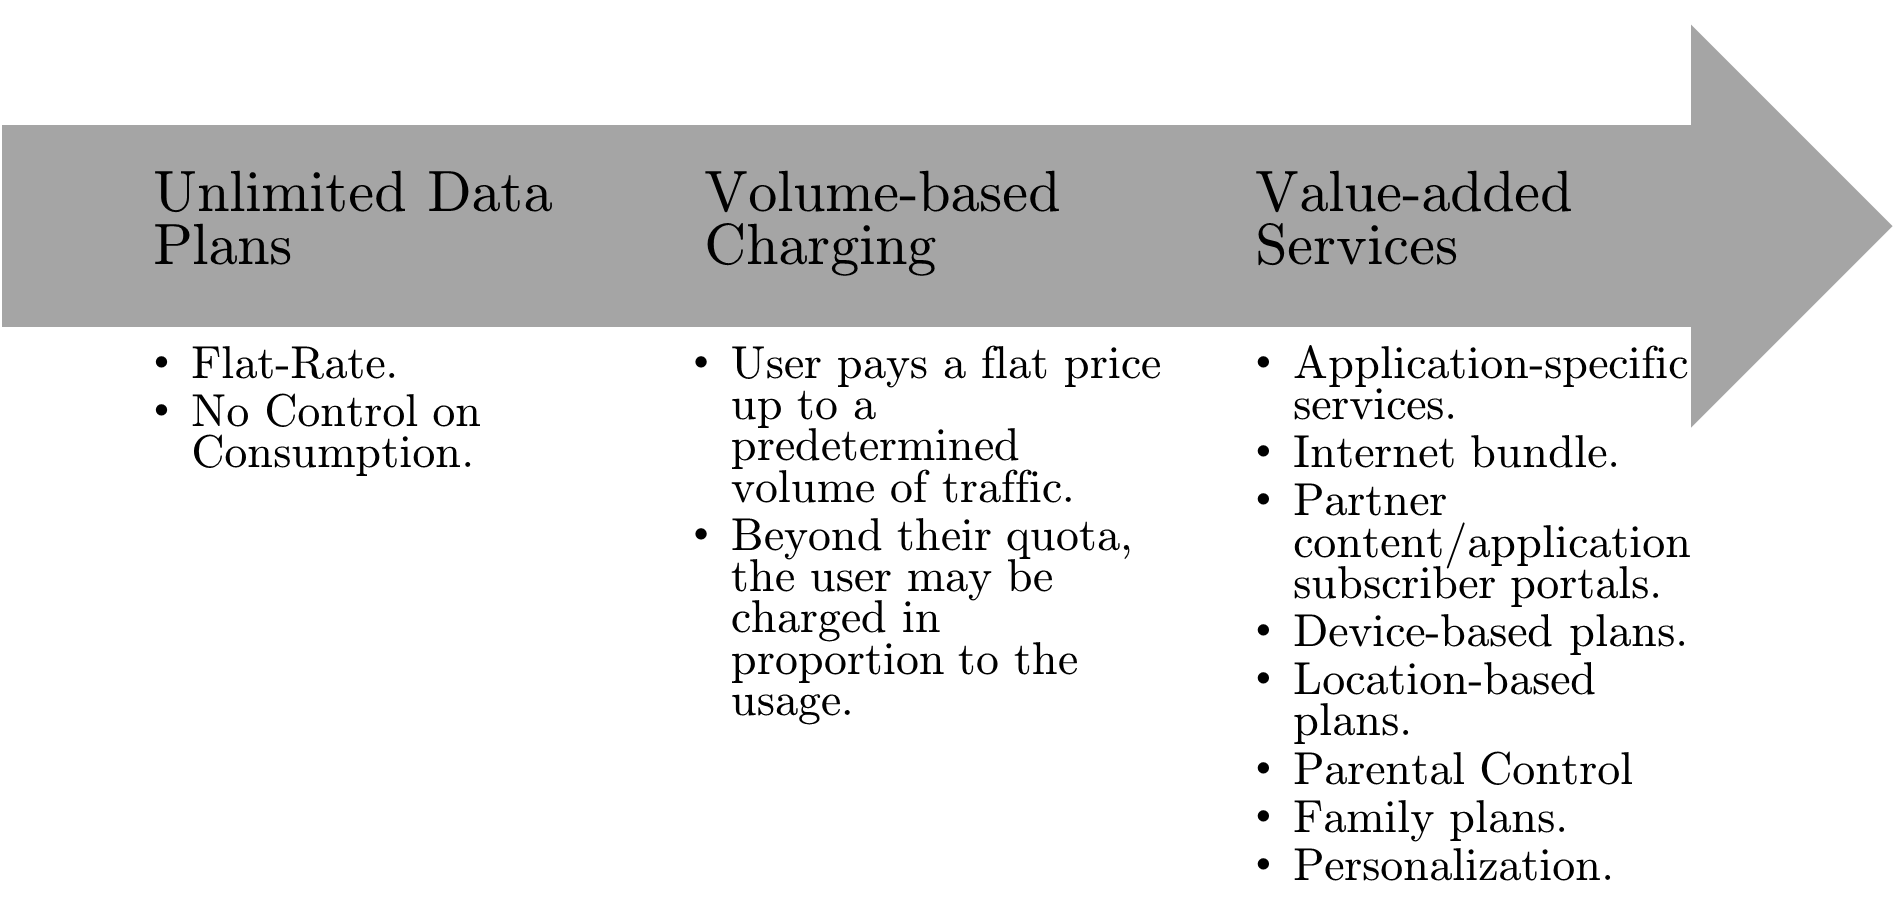
\includegraphics[width=1.00\textwidth]{image/Evolution}
\caption{Evolution of the Mobile Broadband services \cite{Kimbler2012}}
\end{figure}

Later in 2013, Hart and Brown defined similar services to be enabled on an LTE network: Fair usage, Time of Day, Parental Control, Shared Data Plans, Turbo Boost, Bundling of Popular Services (e.g. Twitter, Facebook, etc.) and HD Voice and Video \cite{Hart2013}.\\

Similarly to the authors mentioned above, telecommunication companies have also published their research regarding this topic. For example in 2012, Elitecore Technologies listed a number of emerging use cases, such as: turbo boost, family plans, application-based \& device-based plans, service personalization, etc \cite{Elitecore2012}. While Sandvine, which offers solutions to communication service providers (CSPs), talks about: Application-based service tiers and bolt-ons, roaming packages, shared data plans, sponsored connectivity and third-party bundles \cite{Sandvine2014_2}. Nowadays, Alcatel Lucent and Allot Communications, other telecommunication companies, are also offering solutions about application-based charging, turbo boost and Parental Control \cite{Alcatel2014,Allot2014}. \\

It is clear that network operators have already started to create value added data services and specialized packages that can be sold on top of or instead of the traditional tiered volume-based data packages. This approach is allowing operators to create incremental data revenues and effectively monetize their data traffic in an smarter way \cite{Kimbler2012}.

%Agregar principales problemas perdidas, susbcribers de bajos recursos, etc.%
\subsection{Examples of value-added services}
\noindent
The table \ref{usecases} below, provides an overview of some of the most common volume and value added data services available today. The real advantage of value-based data plans is that they are designed to meet the wants and needs of the end-users and customers \cite{Elitecore2012}.
\begin{table}[H]
\begin{center}
\scalebox{0.8}{	
\begin{tabular}{| l || p{6.2cm} | p{8.2cm} |}
\hline
\textbf{Pricing Policy} & \textbf{Description} & \textbf{Example of Global Telco's} \\
 \hline \hline
\emph{Access Network} & Policy based on the access network. e.g. 2G, 3G, 4G, WiFi, WiMax. & AT\&T, Verizon, T-Mobile (USA), Movistar (Colombia), MTS(Russia), Aircel, Celcom, Singtel.   \\ \hline
\emph{Tiered Plans} & Different Quota-based plans with FUP and overage. & AT\&T, Verizon, T-Mobile (USA), Celcom, Movistar (Colombia), Singtel, Aircel, Vodafone (India).    \\ \hline
 \emph{Device-based plans} & Plans based on the accessed device. e.g. iPad, iPhone, Smart TV, Laptop & AT\&T, Verizon, T-Mobile (USA),Celcom, Movistar (Colombia), MTS(Russia), Aircel, Singtel. \\ \hline
 \emph{Parner-based plans} & Partner-based plans enable operators offer content at subsidized rate. & AT\&T, Verizon, T-Mobile (USA), Maxis, Celcom, SingTel, Aircel, Vodafone (India). \\ \hline
 \emph{Parner-based plans} & Partner-based plans enable operators offer content at subsidized rate. & AT\&T, Verizon, T-Mobile (USA), Maxis, Celcom, SingTel, Aircel, Vodafone (India). \\ \hline
 \emph{Time-based plans} & Time of day, hourly plans, Seasonal plans. & AT\&T, Movistar (Colombia), MTS (Russia), Maxis, Celcom. \\ \hline
 \emph{Service Personalization} & Subscribers can self select from webselfcare. & AT\&T, Verizon, T-Mobile (USA), Movistar (Colombia), MTS (Russia), Maxis, SingTel, Aircel. \\ \hline
 \emph{Parental Control} & Quota management or Application control for child account. & AT\&T, Verizon, Verizon, Maxis.\\ \hline
 \emph{Application/Service} & Application specific charges, e.g. Social networking bundles, emails, etc. & Movistar (Colombia), Maxis, Celcom, SingTel.\\ \hline
 \emph{Family-based Plans} & Data plans with common data pool and sharing & T-Mobile (USA).\\ \hline
\end{tabular}}
\end{center}
\caption{Key use-cases listed by \emph{Elitecore Technologies} in \cite{Elitecore2012}. }
\label{usecases}
\end{table}

\section{Broadband communications technologies}
\noindent
Conflicts among policy rules within a particular plan are the core focus of this thesis. However, the interaction between technologies and the offered services should be well understood. Essentially, all plans are built on top of technologies.\\ 

In order to offer value-added services, network operators need powerful tools to inspect, measure and analyze data traffic in more sophisticated ways that they have done in the past. \\

Several leading vendors including Comverse, Sandvine, Openet, Allot, Huawei and Amdocs have seized this market opportunity and offer comprehensive data traffic management solutions that combine:
  \begin{itemize}
      \item Policy Control (PCRF/PCEF).
      \item Deep Packet Inspection (DPI).
      \item On-line Data Rating and Charging.
	  \item Bandwidth Control and QoS Management.
      \item Content Filtering, Caching and Compression.
	  \item Business Intelligence and Analytics.
    \end{itemize} \bigskip

In the past, many operators used technologies like policy management or DPI to solve specific problems with network congestion, assure fair usage and satisfy regulatory requirements, but they rarely used them to generate new revenue streams \cite{Kimbler2012}.\\	

Operators are showing early interest in using a combination of DPI and policy management to offer value-added services on top of their existing basic packages.

\section{Model Checking}
\noindent
A model can be seen as a simplification of reality. We build models to better understand things, and most importantly, to describe part of a system from a particular perspective. Additionally, a model let us describe unambiguously the system itself or its properties. In this section, we focus on modeling languages and how can we prove or disprove the correctness of it with regards to a specification. \\

A modeling language is any artificial language that can be used to express information or knowledge or systems in a structure that is defined by a consistent set of rules. One of the key benefits of using a modeling language, is that it will let us verify it formally against a given specification. \\ 

Formal verification is the process of applying a manual or automatic formal technique for establishing whether a given system satisfies a given property or behaves in accordance to some abstract description (formal specification) of the system. This verification is done by software tools as model checkers. A model checker thoroughly explores the state space to decide whether the system satisfies the set of properties. \\

Figure \ref{modelChecking} below, illustrates the overall process of Model Checking \cite{Chan1998}. In a first step, which is called modeling, the system description is converted into the system model. The requirements have to be manually formalized because they are mostly given in natural language. The result of this formalization is the formal specification given as formulas in a temporal logic such as LTL (Linear Temporal Logic). \\

As shown below, the model and the specification are inputs given to the model checker. The model checker uses an exhaustive search over all reachable states of the model to check whether the model satisfies the formula. In the end, it returns a result. The result may be that the model satisfies the formula or that the model does not satisfy the formula.  \\

\begin{figure}[H]
\centering
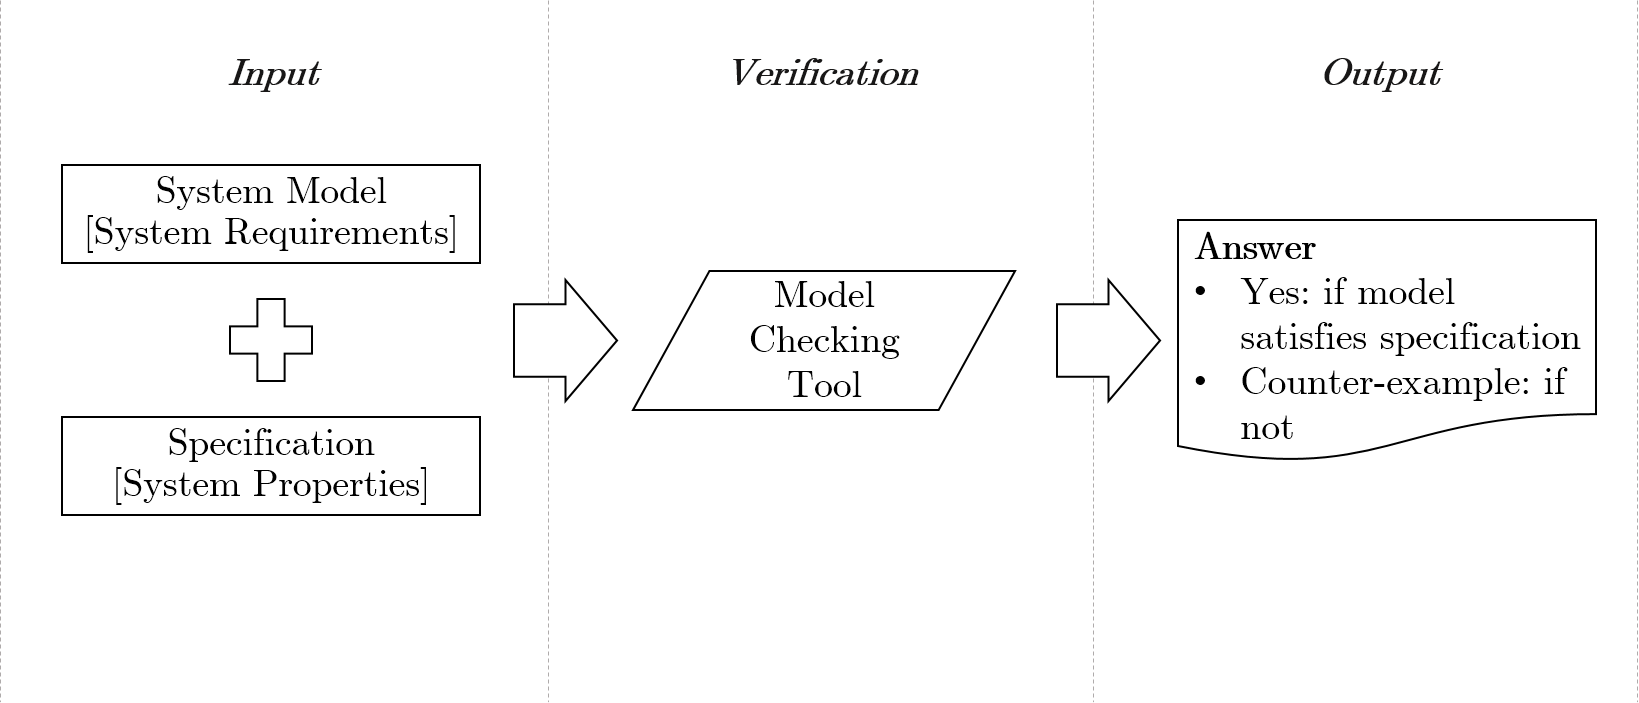
\includegraphics[width=0.95\textwidth]{image/ModelChecking}
\caption{Model checking process}
\label{modelChecking}
\end{figure}

\bigskip

\subsection{Spin Model Checker and PROMELA}
\noindent
Spin and most of its predecessors are implementations of standard automata-based reachability analyzers, with primary emphasis on performance. It provides an efficient implementation of a classic reachability analyzer with a firm and well-understood theory for LTL model checking \cite{holzmann2000spin} - or also known as the VardiWolper framework for automata-theoretic verification \cite{Vardi1986}. It supports the use of LTL (linear temporal logic) for the specification of correctness properties.\\

Spin accepts specifications written in a meta-language named Promela (Process Meta Language). Promela is a verification modeling language introduced by Gerard J. Holzmann. The language allows for the dynamic creation of concurrent processes to model, for example, concurrent or distributed systems. The three main types of objects that can be manipulated are: 
  \begin{itemize}
      \item processes,
      \item channels, and
      \item variables. 
    \end{itemize} \bigskip

Spin represents the system as a finite state machine. It visits each reachable state explicitly using Nested DFS and using partial order reduction. If a property is specified in LTL, Spin will first convert the LTL formula into an equivalent never claim, using the procedure outlined in \cite{Gerth1995}. Formally, the never claim specifies a Buchi automaton (a specific type of omega automaton) and the acceptance conditions from this automaton are evaluated on the global systems execution graph \cite{holzmann2000spin}. The efficiency of the Spin system comes from its on-the-fly procedure for performing this check that requires only small amounts of memory to be consumed for each state that is reached. The details of this so-called nested depth-first search algorithm are documented in \cite{Holzmann1996}. 

\subsubsection{Data Types}
\noindent
In Promela, there are seven predefined integer data types: bit, bool, byte, pid, short, int, and unsigned . There are also constructors for user-defined data types, and there is a separate predefined data type for message passing channels. Variables of type bit and bool are stored in a single bit of memory, which means that they can hold only binary, or boolean values.  \\

Typedef declarations can be used to introduce user-defined data types. User-defined data types can use any predefined integer data types. 

\subsection{Linear Temporal Logic - LTL}
\noindent
Spin, as any other model checker, needs a number of system properties to verify the System Model (expressed in Promela). Without the system properties, the model checker cannot really tell whether or not the System Model is correct. In Promela, Linear Temporal Logic is used for specifying the correctness of requirements. \\

Linear temporal logic (LTL) is a modal temporal logic with modalities referring to time. In LTL, one can encode formulas about the future of paths, e.g. a condition will eventually be true, a condition will be true until another fact becomes true, etc. It is a fragment of the more complex CTL*, which additionally allows branching time and quantifiers. 
\clearpage
LTL is built up from a finite set of propositional variables, logical operators (i.e. $\neg$, $\land$, $\lor$, $\implies$, $\iff$, \emph{true} and \emph{false}), and four additional temporal modal operators.

\begin{table}[H]
\begin{center}
\scalebox{0.8}{	
\begin{tabular}{| l || l | l |}
\hline
\textbf{LTL Formula} & \textbf{Description} & \textbf{Semantics Meaning} \\
 \hline \hline
$\square$ $\phi$ & Always & $\phi$ is satisfied at every state. \\ \hline
$\lozenge$ $\phi$ & Eventually & $\phi$ is satisfied at some state. \\ \hline
$\psi$ U $\phi$ & Until & $\psi$ has to hold at least until $\phi$, which holds at the current or a future position. \\ \hline
X $\phi$ & Next & $\phi$ has to hold at the next state. \\ \hline
\end{tabular}}
\end{center}
\caption{Semantics for the temporal operators}
\label{tem_operators}
\end{table}

An important taxonomy of properties, as given below, is found in many books and papers \cite{Schneider2004}. Safety and liveness properties described below, are of our particular interest; as most of our specifications are safety and liveness properties. \\

\emph{Safety properties} state that for all computations of the system, and for all instances of time, some property will invariantly hold. Colloquially, Safety properties assert that something \textquotedblleft bad\textquotedblright never happens. For example, a safety property could be defined as: \emph{Facebook traffic will never be blocked}. \\

\emph{Liveness properties} state that some desired state of the system can eventually be reached. Colloquially, a Liveness property makes sure that something \textquotedblleft good\textquotedblright  eventually happens. An example of a liveness property could be: \emph{If any other traffic is generated, it will eventually be blocked}. \\

\emph{Persistence properties} are related to the stabilization of certain properties. In general, a persistence property describes that for all possible computations, there is a point of time when a certain property will always hold afterwards. For example: there is a point where rule A is always enabled.\\

\emph{Fairness properties} state that some property will hold infinitely often. For example: No process is ignored infinitely often by an O.S. 
\section{Related Work}
\noindent
Model checking, or property checking, has been widely used in many other domains to exhaustively and automatically check whether a given model meets a given specification. Our primary interest is the use of Promela as the Model Checking tool to detect conflicts, via LTL formulas, in rules-based plans. \\

One of the main contributions for this Thesis is the research done by Zhiping Duan in 2003 \cite{Duan2003}. In his work, he provides an approach to automatically detect feature interactions (i.e. conflicts) in telecommunications systems, which are not essentially rules-based. Even though, Duan uses LTL and FOL (First-Order-Logic) to prove their systems, he proposed an implementation of a FOL prover in $\lambda$Prolog. We think it is more intuitively to use Promela for our particular domain, as Promela is a verification modeling language which directly allows LTL formulas for its verification. \\

In 2007, Antoniou, et al, integrate several aspects of policy specification languages (i.e. rule-based reasoning), in a common framework. One key contribution from his research to our Thesis, is the use of priorities to resolve conflict among rules. In his research, the implementation of a conflict checker was not addressed. \\

Between 2010 and 2011, several requirements frameworks for business process compliance management have been proposed. In \cite{Abramowicz2010,Hantry2011}, the authors formulate requirements for compliance rules. The requirements address the issues of lifetime compliance. The focus is also on the requirements to languages expressing compliance rules, on the rules priority, and on validation of process models against rules during design time and runtime. \\

In 2012, Gawanmeh, et al, proposed a novel algorithm for detecting conflicts in firewall rules \cite{Gawanmeh2012}. Even though his novel approach, using domain restriction, is interesting; its proposed algorithm doesn't consider rules with multiple types of conditions. \\

The review of the related work above, illustrates that the problem of conflicts among rules exists in different domains and, more importantly, Model-Checking is a proven approach for detecting the conflicts efficiently. In this Thesis, we will use Promela to detect conflicts in a particular area of telecommunications: rule-based Internet Plans. \\ 

\section{Summary of the chapter}
\noindent
The literature review is summarized below:
   \begin{itemize}
      \item Network Operators are basically moving from unlimited or volume-based models to value-added data offerings. These value-added services comprise a number of custom rules to form a Plan. 
      \item Because all of these services are built on top of technologies, there are a number of technical, commercial, regulatory or integration impacts, that needs to be considered when designing these value-added services. 
      \item Model Checking can perfectly be used to exhaustively and automatically verify whether a model meets a given specification. In our case the rule-based plans will be modeled using Promela and the specification will be defined in LTL. 
	  \item The problem of conflicts among rules has been studied in many other domains and, more importantly, Model-Checking is a proven approach for detecting the conflicts efficiently.
	  \item In this Thesis, Promela will be used to detect conflicts in a particular area of telecommunications: rule-based Plans.
    \end{itemize} \bigskip

In the next chapter, we will introduce the model proposed for specifying the rule-based plans and will expand on the LTL properties to verify the proposed model. \\

\clearpage